\documentclass[a4paper,12pt,obeyspaces,spaces,hyphens]{article}

\def \trainingtitle{Formation développemment Linux embarqué avec Buildroot}
\def \trainingduration{Séminaire en ligne, 5 sessions de 4 heures}

\usepackage{agenda}

\renewcommand{\arraystretch}{2.0}

\begin{document}

\setlength{\arrayrulewidth}{0.8pt}

\feshowtitle

\small
\newcolumntype{g}{>{\columncolor{fedarkblue}}m{4cm}}
\newcolumntype{h}{>{\columncolor{felightblue}}X}

\arrayrulecolor{lightgray} {
  \setlist[1]{itemsep=-5pt}
  \begin{tabularx}{\textwidth}{|g|h|}
    {\bf Titre} & {\bf Formation développement Linux embarqué avec Buildroot} \\
    \hline

    {\bf Thématiques} &
    Introduction à Buildroot \par
    Gérer et compiler une configuration \par
    Arborescence des sources et des fichiers générés \par
    Gestion de la configuration du noyau Linux avec Buildroot \par
    Système de fichiers racine \par
    Infrastructure de téléchargement \par
    Introduction à GNU Make \par
    Ajout de nouveaux paquets \par
    Aspects avancés sur les paquets Buildroot \par
    Analyse du build \par
    Sujets avancés \par
    Développement d’application avec Buildroot \par
    Comprendre le fonctionnement interne de Buildroot \par
    Communauté Buildroot: obtenir du support et contribuer \par
    Quoi de neuf dans Buildroot ? \\
    \hline
    {\bf Supports} &
    Vérifiez que le contenu de la formation correspond à vos besoins :
    \newline \url{https://bootlin.com/doc/training/buildroot}. \\
    \hline

    {\bf Durée} & {\bf Cinq} demi-journées - 20 h (4 h par demi-journée)
    \newline 80\% de présentations et 20\% de démonstrations. \\
    \hline

    {\bf Formateur} & {\bf Thomas Petazzoni}. Thomas est un des quatre
    co-mainteneurs du projet Buildroot. Il participe au projet depuis
    2009, et y a contribué près de 5000 patches.\\
    \hline

    {\bf Langue} & Présentations : Français
    \newline Supports : Anglais\\
    \hline

    {\bf Public ciblé} & Sociétés qui utilisent déjà Buildroot ou qui
    sont intéressées par l'utiliser pour construire leurs systèmes Linux
    embarqué.\\
    \hline

    {\bf Pré-requis} & {\bf Connaissance de Linux embarqué}, sujet couvert par
    notre formation Linux embarqué :
    \url{https://bootlin.com/training/embedded-linux/} \vspace{1em}
    \newline {\bf Connaissance et pratique des commandes UNIX ou
    GNU/Linux}
    \newline Les personnes n'ayant pas ces connaissances peuvent
    s'autoformer, par exemple en utilisant nos supports de formation
    disponibles en ligne :
    \newline (\url{https://bootlin.com/blog/command-line/}) \\
    \hline
  \end{tabularx}

  \begin{tabularx}{\textwidth}{|g|h|}
    {\bf Équipement nécessaire} &
    \begin{itemize}
    \item Ordinateur avec le système d'exploitation de votre choix, équipé du
          navigateur Google Chrome ou Chromium pour la conférence vidéo.
    \item Une webcam et un micro (de préférence un casque avec micro)
    \item Une connexion à Internet à haut débit
    \end{itemize}\\
    \hline

    {\bf Supports} & Version électronique des présentations, des instructions
   et des données pour les démos.\\
    \hline

\end{tabularx}}
\normalsize

\feagendatwocolumn
{Matériel}
{
  La plateforme matérielle utilisée pendant les démonstrations pratiques de
  cette formation est la carte {\bf BeagleBone Black}, dont voici les
  caractéristiques :

  \begin{itemize}
  \item Un processeur ARM AM335x de Texas Instruments (à base de
    Cortex-A8), avec accélération 3D, etc.
  \item 512 Mo de RAM
  \item 2 Go de stockage eMMC embarqué sur la carte
	\newline(4 Go avec la révision C)
  \item USB hôte et device
  \item Sortie HDMI
  \item Connecteurs à 2 x 46 broches, pour accéder aux UARTs, aux
        bus SPI, aux bus I2C, et à d'autres entrées/sorties du
        processeur.
  \end{itemize}
}
{}
{
  \begin{center}
    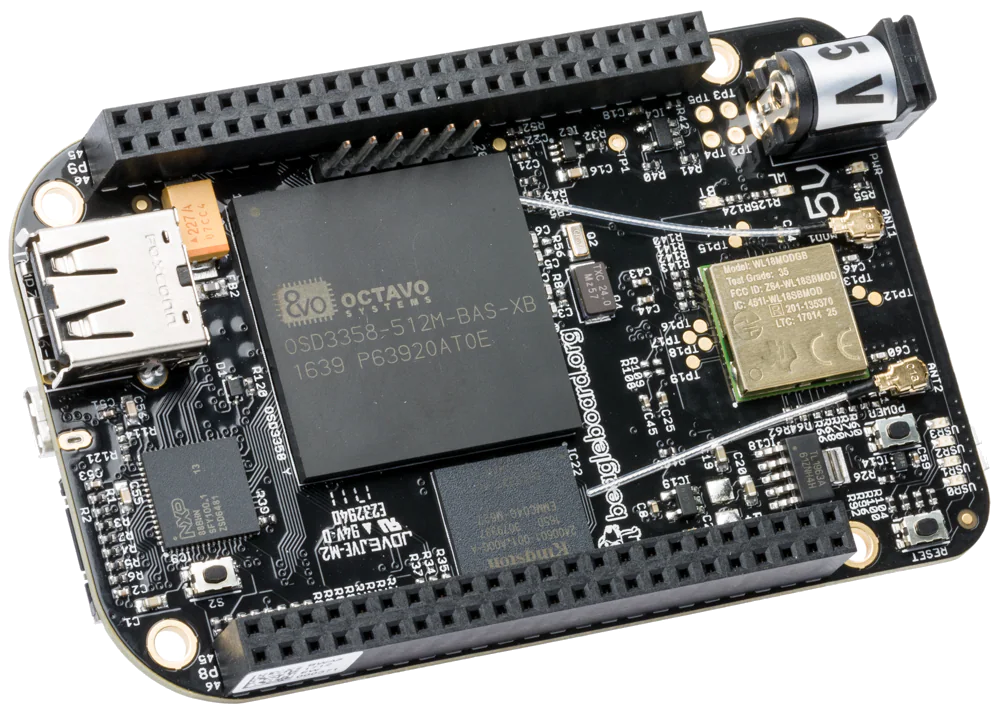
\includegraphics[height=5cm]{../slides/beagleboneblack-board/beagleboneblack.png}
  \end{center}
}

\section{1\textsuperscript{ère} demi-journée}

\feagendatwocolumn
{Cours - Introduction à Buildroot et aux systèmes de build}
{
  \begin{itemize}
  \item Architecture générale d'une système Linux embarqué
  \item Choix entre systèmes de build et distributions binaires
  \item Rôle d'un système de build
  \item Comparaison des systèmes de build existants
  \end{itemize}
}
{Cours - Présentation de Buildroot}
{
  \begin{itemize}
  \item Points clés autour du projet
  \item Téléchargement des sources de Buildroot
  \item Configuration simple de Buildroot
  \item Exécution d'une premières compilation
  \end{itemize}
}
\\
\feagendatwocolumn
{Démo - Utilisation simple de Buildroot}
{
  \begin{itemize}
  \item Téléchargement et configuration de Buildroot
  \item Configurer et compiler un système simple avec Buildroot, pour la
        carte BeagleBone Black
  \item Flasher et tester le système générer sur la carte BeagleBone
        Black.
  \end{itemize}
}
{Cours - Gestion de la compilation et de la configuration}
{
  \begin{itemize}
  \item Compilation en dehors des sources
  \item Utiliser et créer des fichiers {\em defconfigs}
  \item Fragments de {\em defconfigs}
  \item Autres astuces pour la compilation
  \end{itemize}
}

\feagendaonecolumn
{Cours - Sources de Buildroot et arborescence des fichiers générés}
{
  \begin{itemize}
  \item Détails sur l'organisation du code source de Buildroot
  \item Détails sur l'arborescence des fichiers générés
  \end{itemize}
}

\section{2\textsuperscript{ème} demi-journée}

\feagendaonecolumn
{Cours - Chaînes de compilation {\em toolchains} dans Buildroot}
{
  \begin{itemize}
  \item Les différents possibilités d'usage de chaînes de compilation
	dans Buildroot.
  \item Tour d'horizon des options liées aux chaînes de compilation.
  \item Utilisation de chaînes des compilation binaires, comme
	celles de Bootlin. Détails sur les fonctionnalités
        {\em multilib} et l'intégration des toolchains dans Buildroot.
  \item Génération de toolchains sur mesure avec {\em Crosstool-NG},
	et leur utilisation comme chaînes externes.
  \end{itemize}
}

\feagendatwocolumn
{Cours - Gestion de la configuration du noyau Linux}
{
  \begin{itemize}
  \item Charger, modifier et sauvegarder la configuration du noyau.
  \end{itemize}
}
{Cours - Construction du système de fichier racine dans Buildroot}
{
  \begin{itemize}
  \item Comprendre comment Buildroot construit le système de fichiers
	racine: {\em skeleton}, installation de composants, {\em
        overlays}, scripts {\em post-build} et {\em post-image}.
  \item Personnalisation du contenu du système de fichiers
  \item Configuration du système: sélection de la {\em console},
	plusieurs méthode de gestion de {\tt /dev}, les différentes
	implémentations d'{\tt init}, etc.
  \item Comprendre comment Buildroot génère les images de systèmes de
	fichiers.
  \end{itemize}
}

\feagendaonecolumn
{Démo - Personnalisation du système de fichiers}
{
  \begin{itemize}
  \item Exploration des fichiers générés
  \item Personnalisation du système de fichiers racine en utilisant un {\em rootfs overlay}
  \item Personnaliser le noyau avec des correctifs et des options de
	configuration supplémentaires
  \item Rajout de nouveaux composants
  \item Utilisation de fichiers {\em defconfig} et compilation en
	dehors des sources.
  \end{itemize}
}

\feagendaonecolumn
{Cours - Infrastructure de téléchargement dans Buildroot}
{
  \begin{itemize}
  \item Méthodologie de téléchargement
  \item Site primaire et sites de backup, compilation en mode déconnecté
  \item Téléchargement via systèmes de contrôle de versions,
	vérification d'intégrité
  \item Cibles {\em make} en rapport avec les téléchargements
  \end{itemize}
}

\section{3\textsuperscript{ème} demi-journée}

\feagendaonecolumn
{Cours - Introduction à GNU Make}
{
  \begin{itemize}
  \item Éléments de base des règles de make
  \item Définition et utilisation de variables
  \item Conditions et fonctions
  \item Écriture de recettes
  \end{itemize}
}

\feagendatwocolumn
{Cours - Intégration de nouveaux composants dans Buildroot}
{
  \begin{itemize}
  \item Comment rajouter de nouveaux paquetages au système de
	configuration de Buildroot
  \item Comprendre les différentes infrastructures de paquetages : pour
	des composants {\em generic}, {\em autotools}, {\em CMake}, {\em
	Python} et autres
  \item Écriture un fichier \code{Config.in} pour un composant: comment
    exprimer des dépendances vers d'autres composants, vers des options
    de toolchains, etc.
  \item Détails sur l'écriture d'une recette pour un composant :
	description de l'emplacement du code source, de la méthode de
	téléchargement, de configuration, de compilation et
	d'installation, gestion des dépendances, etc.
  \end{itemize}
}
{Démo - Nouveaux composants dans Buildroot}
{
  \begin{itemize}
  \item Création d'un nouveau paquetage pour {\em nInvaders}
  \item Comprendre comment rajouter des dépendances
  \item Ajouter des correctifs pour {\em nInvaders} pour prendre en
	charge le contrôle via un {\em Nunchuk}
  \end{itemize}
}

\feagendaonecolumn
{Cours - Notions avancées sur les paquetages}
{
  \begin{itemize}
  \item Rapport de licences
  \item Prise en charge des correctifs: ordre d'application et format,
	répertoire global pour les correctifs, etc.
  \item Utilisateur, droit d'accès, tables de fichiers devices
  \item Script d'init et fichiers unitaires pour systemd
  \item Scripts de configuration
  \item Compréhension des {\em hooks}
  \item Surcharger des commandes
  \item Gestion des paquetages legacy
  \item Paquetages virtuels
  \end{itemize}
}

\section{4\textsuperscript{ème} demi-journée}

\feagendaonecolumn
{Démo - Paquetages avancés}
{
  \begin{itemize}
  \item Packager une application avec une dépendance obligatoire et
    une dépendance optionnelle
  \item Packager une bibliothèque, hébergée sur GitHub
  \item Utilisation de {\em hooks} pour ajuster les paquetages
  \item Rajouter un correctif à un paquetage
  \end{itemize}
}

\feagendatwocolumn
{Cours - Analyse d'une compilation: licences, dépendances, temps de
construction}
{
  \begin{itemize}
  \item Utilisation de l'infrastructure de gestion des informations
	légales
  \item Représentation graphique des dépendances entre paquetages
  \item Collecte d'informations et représentation du temps de
	compilation
  \end{itemize}
}
{Cours - Sujets avancés}
{
  \begin{itemize}
  \item \code{BR2_EXTERNAL} pour stocker des personnalisations à
	l'extérieur des sources de Buildroot
  \item Cibles make spécifiques pour les paquetages
  \item Comprendre les recompilations
  \item Astuces pour compiler plus vite
  \end{itemize}
}

\feagendaonecolumn
{Démo - Sujets avancés}
{
  \begin{itemize}
  \item Utilisation des capacités de génération de graphes de temps de
	compilation
  \item Génération de graphes de dépendances
  \item Utilisation du rapport sur les licences, et ajout d'informations
	légales à vos propres paquetages
  \item Utilisation de \code{BR2_EXTERNAL}
  \end{itemize}
}

\section{5\textsuperscript{ème} demi-journée}

\feagendatwocolumn
{Cours - Développement applicatif avec Buildroot}
{
  \begin{itemize}
  \item Utilisation de Buildroot pendant le développement d'applications
  \item Utilisation de l'environnement de Buildroot pour compiler des
	applications en dehors de Buildroot
  \item Générer un SDK pour d'autres développeurs
  \item Débug à distance avec Buildroot
  \end{itemize}
}
{Démo - Développement applicatif avec Buildroot}
{
  \begin{itemize}
  \item Compiler et exécuter votre propre application
  \item Débug à distance de votre application
  \item Utilisation de \code{<pkg>_OVERRIDE_SRCDIR}
  \end{itemize}
}

\feagendatwocolumn
{Cours - Comprendre les mécanismes internes de Buildroot}
{
  \begin{itemize}
  \item Description détaillée du processus de compilation de Buildroot:
    	toolchain, paquetages, construction du système de fichiers race,
	fichiers {\em stamp}, etc.
  \item Comprendre les paquetages virtuels.
  \end{itemize}
}
{Cours - Obtenir de l'aide et s'impliquer, nouveautés dans Buildroot}
{
  \begin{itemize}
  \item Obtenir de l'assistance technique: {\em Bugzilla}, {\em liste de
	discussion}, {\em IRC}
  \item Contribuer: comprendre le processus de développement, comment
    soumettre des correctifs
  \item Nouveautés dans Buildroot: résumé des principaux changements
    depuis les deux dernières années
  \end{itemize}
}

\feagendaonecolumn
{Questions / réponses}
{
  \begin{itemize}
  \item Questions et réponses avec les participants à propos des sujets abordés.
  \item Présentations supplémentaires s'il reste du temps, en fonction des demandes
        de la majorité des participants.
  \end{itemize}
}

Note: la dernière session peut être plus courte que les autres
sessions et se terminer plus tôt, selon le nombre de questions des
participants.

\end{document}
